\chapter{Wechselstromtechnik}

\section{Komplexe Zahlen}
Komplexe Zahlen sind die Erweiterung der Realen Zahlen $\mathbb{R}$:
\begin{align}
    \mathbb{N}\rightarrow\mathbb{Z}\rightarrow\mathbb{R} (\mathbb{Q}+\mathbb{I})\rightarrow\mathbb{C}
\end{align}

Die Defintion $j=\sqrt{-1}$ ist hierbei besonders wichtig.

\vspace{0.5cm}

\subsubsection*{Beispiel}
\begin{align}
    &x^2=-9         \\
    &x^2=j^2\cdot 9\hspace{0.25cm}|\sqrt{}\\
    &\Rightarrow x_1=3j\hspace{0.5cm} x_2=-3j
\end{align}

\newpage

Eine komplexe Zahl $\underline{z}$ besteht aus einem Realteil $a$ und einem Imaginärteil $b$

\begin{center}
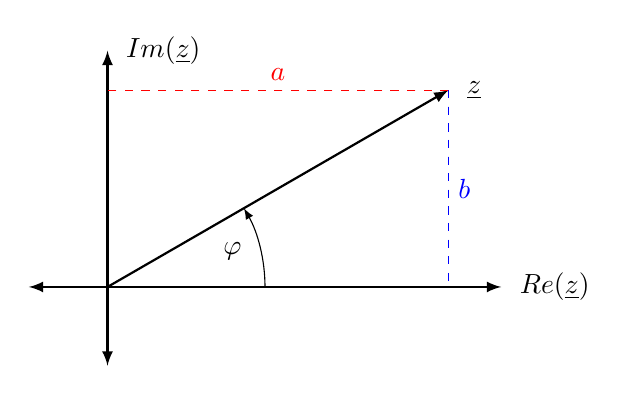
\begin{tikzpicture}[>=latex]
    \draw[style=help lines] (0,0) (3,2);

    \coordinate (pointer) at (30:5); 
    % \coordinate (vec2) at (30:2.5);
    \coordinate (posX) at (0:5);
    \coordinate (posY) at (90:3);
    \coordinate (negX) at (180:1);
    \coordinate (negY) at (270:1);

    \draw[->,thick,black] (0,0) -- (pointer) node[right, xshift=3pt] {$\underline{z}$};
    % \draw at (15:2.5) node[left,top,xshift=3pt,yshift=3pt] {$\underline{|z|}$};
    \draw[->,thick,black] (0,0) -- (posX) node[right,xshift=3pt] {$Re(\underline{z})$};
    \draw[->,thick,black] (0,0) -- (posY) node[right,xshift=3pt] {$Im(\underline{z})$};
    \draw[->,thick,black] (0,0) -- (negX);
    \draw[->,thick,black] (0,0) -- (negY);

    % Re
    \draw[dashed,red] (pointer) -- +(-{sin(60)*5},0);
    \draw[dashed,red] (pointer) -- +(-{sin(60)*5}/2,0) node[above] {$a$};

    % Im
    \draw[dashed,blue] (pointer) -- +(0,-{sin(30)*5});
    \draw[dashed,blue] (pointer) -- +(0,-{sin(30)*5}/2) node[right] {$b$};

    \draw[->] (2,0) arc (0:30:2) node[midway,left,xshift=-3pt,yshift=-2pt] {$\varphi$};
\end{tikzpicture}
\end{center}

Der Betrag des Zeigers ($|\underline{z}|$) ist die Länge, $\varphi$ der Winkel zwischen der x-Achse und dem Zeiger.
\begin{align}
    &\underline{z}=a+jb=Re(\underline{z})+j Im(\underline{z})   \\
    &\underline{z}=|\underline{z}|\cdot e^{j\varphi}
\end{align}
Die Länge kann über den Pythagoras berechnet werden und der Winkel mit dem Arkustangens:
\begin{align}
    Re(\underline{z})&=|\underline{z}|\cdot cos(\varphi)                \\
    Im(\underline{z})&=|\underline{z}|\cdot sin(\varphi)                \\
    \varphi&=arctan(\frac{Im(\underline{z})}{Re(\underline{z})})        \\
    |\underline{z}|&=\sqrt{Re(\underline{z})^{2}+Im(\underline{z})^{2}}
\end{align}

\newpage

\subsection{Addition \& Subtraktion}
Die Summe \& Differenz kompler Zahlen $\underline{z_1}=a+jb$ und $\underline{z_2}=c+jd$ ist definiert als
\begin{align}
    \underline{z_1} + \underline{z_2} = (a+c) + j(b+d) \hspace{1cm} \underline{z_1} - \underline{z_2} = (a+c) - j(b+d)
\end{align}

Es werden Real- und Imaginärteile addiert bzw. subtrahiert.\\

Grafisch können Zahlen in Zeigerdarstellung wie Vektoren addiert bzw. subtrahiert werden. D.h. beim Addieren wird das Ende eines Zeigers an die Spitze des anderen gehängt.\\

\underline{Beispiel} \\
$\underline{x} = 3 \cdot e^{j \cdot 30\degree}$ \\
$\underline{y} = 3 \cdot e^{j \cdot 240\degree}$ \\

Gesucht: $\underline{z}$\\
$\underline{z}=\underline{x}+\underline{y}$

\begin{center}
\begin{tikzpicture}[>=latex]
    \draw[style=help lines] (0,0) (3,2);

    \coordinate (pointer0) at (30:3);
    \coordinate (pointer1) at (240:3);
    \coordinate (posX) at (0:3);
    \coordinate (posY) at (90:2);
    \coordinate (negX) at (180:1);
    \coordinate (negY) at (270:2);

    \draw[->,thick,red] (0,0) -- (pointer0) node[right, xshift=3pt, red] {$\underline{x}$};
    \draw[->,thick,blue] (pointer0) -- +(pointer1) node[right, xshift=3pt, blue] {$\underline{y}$};
    \draw[->,thick,teal] (0,0) -- ($(pointer0) + (pointer1)$) node[below left, xshift=3pt, teal] {$\underline{z}$};

    \draw[->,thick,black] (0,0) -- (posX) node[right,xshift=3pt] {$Re(\underline{z})$};
    \draw[->,thick,black] (0,0) -- (posY) node[right,xshift=3pt] {$Im(\underline{z})$};
    \draw[->,thick,black] (0,0) -- (negX);
    \draw[->,thick,black] (0,0) -- (negY);
\end{tikzpicture}
\end{center}

\newpage

\subsection{Multiplikation}
Die Längen der Zeiger multiplizieren und die Winkel addieren:
\begin{align}
    \underline{y}\cdot\underline{z}=|\underline{y}|\cdot|\underline{z}|\cdot e^{j\cdot(\varphi_{\underline{y}}+\varphi_{\underline{z}})}
\end{align}

\subsection{Division}
Die Längen der Zeiger dividieren und die Winkel subtrahieren:
\begin{align}
    \frac{\underline{y}}{\underline{z}}=\frac{|\underline{y}|}{|\underline{z}|}\cdot e^{j\cdot(\varphi_{\underline{y}}-\varphi_{\underline{z}})}
\end{align}

\subsection{Konjugiert Komplexe Zahlen}
Konjugiert-Komplexe Zahlen sind besonders wichtig, wenn man mit komplexen Zahlen rechnen möchte. Um die konjugiert-komplexe Zahl zu ermitteln, wird nur das Vorzeichen des Imaginärteils der Zahl umgedreht; sie wird als $\underline{z}^*$ angeschrieben.
\begin{align}
    \underline{z}&=a+jb=|\underline{z}|\cdot e^{j\varphi}       \\
    \underline{z}^*&=a-jb=|\underline{z}|\cdot e^{-j\varphi}
\end{align}

Visuell ist es das Gleiche, als wenn man den Punkt auf der x-Achse spiegelt.

\begin{center}
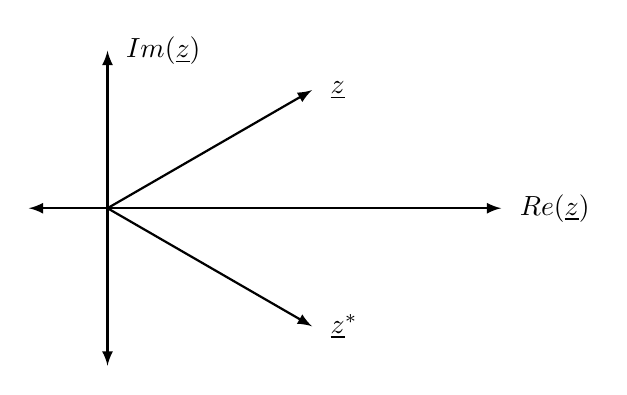
\begin{tikzpicture}[>=latex]
    \draw[style=help lines] (0,0) (3,2);

    \coordinate (pointer) at (30:3);
    \coordinate (negPointer) at (330:3);
    % \coordinate (vec2) at (30:2.5);
    \coordinate (posX) at (0:5);
    \coordinate (posY) at (90:2);
    \coordinate (negX) at (180:1);
    \coordinate (negY) at (270:2);

    \draw[->,thick,black] (0,0) -- (pointer) node[right, xshift=3pt] {$\underline{z}$};
    \draw[->,thick,black] (0,0) -- (negPointer) node[right, xshift=3pt] {$\underline{z}^*$};

    \draw[->,thick,black] (0,0) -- (posX) node[right,xshift=3pt] {$Re(\underline{z})$};
    \draw[->,thick,black] (0,0) -- (posY) node[right,xshift=3pt] {$Im(\underline{z})$};
    \draw[->,thick,black] (0,0) -- (negX);
    \draw[->,thick,black] (0,0) -- (negY);
\end{tikzpicture}
\end{center}

\newpage

\section{Zeigerdiagramm}
Mit Zeigerdiagrammen kann man sinusförmige Funktion übersichtlicher darstellen. Die Zeiger folgen dem Einheitskreis und sollen zeigen, wie sich die Funktion zeitlich verhält.

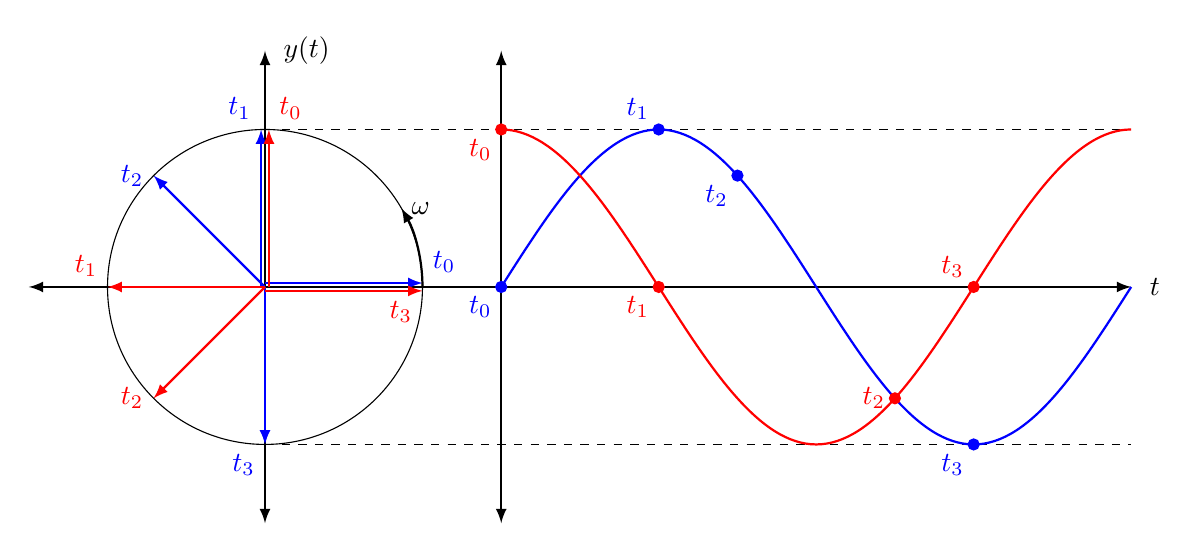
\begin{tikzpicture}[>=latex]
    \draw[style=help lines] (0,0) (3,2);

    % Plot
    \coordinate (posX) at (0:11);
    \coordinate (posY) at (90:3);
    \coordinate (negX) at (180:3);
    \coordinate (negY) at (270:3);

    \draw[->,thick,black] (0,0) -- (posX) node[right,xshift=3pt] {$t$};
    \draw[->,thick,black] (0,0) -- (posY) node[right,xshift=3pt] {$y(t)$};
    \draw[->,thick,black] (0,0) -- (negX);
    \draw[->,thick,black] (0,0) -- (negY);

    \draw[dashed] (90:2) -- +(11,0);
    \draw[dashed] (270:2) -- +(11,0);
    \draw[->,thick,black] (0:3)  -- +(0,3);
    \draw[->,thick,black] (0:3)  -- +(0,-3);

    % Pointer
    \draw[->,thick,blue] (0,0.05) -- +(2,0) node[above right] {$t_0$};
    \draw[->,thick,blue] (-0.05,0) -- +(0,2) node[above left] {$t_1$};
    \draw[->,thick,blue] (0,0) -- (135:2) node[left] {$t_2$};
    \draw[->,thick,blue] (0,0) -- (270:2) node[below left] {$t_3$};

    \draw[->,thick,red] (0.05,0) -- +(0,2) node[above right] {$t_0$};
    \draw[->,thick,red] (0,0) -- (180:2) node[above left] {$t_1$};
    \draw[->,thick,red] (0,0) -- (225:2) node[left] {$t_2$};
    \draw[->,thick,red] (0,-0.05) -- +(2,0) node[below left] {$t_3$};

    % Circle
    \draw[-] (2,0) arc (0:360:2);
    \draw[->, thick] (2,0) arc (0:30:2) node[right] {$\omega$};

    % Sinewave
    \draw[thick, blue] (3,0) sin (5,2) cos (7,0) sin (9,-2) cos (11,0);
    % Cosinewave
    \draw[thick, red] (3,2) cos (5,0) sin (7,-2) cos (9,0) sin (11,2);

    % Points
    \filldraw[blue] (3,0)       circle (2pt) node[below left, blue] {$t_0$};
    \filldraw[blue] (5,2)       circle (2pt) node[above left, blue] {$t_1$};
    \filldraw[blue] (6,1.4142)  circle (2pt) node[below left, blue] {$t_2$};
    \filldraw[blue] (9,-2)      circle (2pt) node[below left, blue] {$t_3$};

    \filldraw[red] (3,2)       circle (2pt) node[below left, red]   {$t_0$};
    \filldraw[red] (5,0)       circle (2pt) node[below left, red]   {$t_1$};
    \filldraw[red] (8,-1.4142) circle (2pt) node[left, red]         {$t_2$};
    \filldraw[red] (9,0)       circle (2pt) node[above left, red]   {$t_3$};
\end{tikzpicture}

\newpage

\section{Impedanz}
Die Impedanz ist der "Widerstand" eines Systems, die aber auch die Frequenz einbezieht (weil der Imaginärteil nicht $0$ ist). Sie wird mit $z$ dargestellt.
\begin{align}
    &\underline{z}=\frac{\underline{U}}{\underline{I}}  \\
    &\underline{z}=R+jx
\end{align}

\subsubsection*{Beispiel}
Kondensator: $C=1\mu F$\\
\begin{align}
    &\underline{z}_C=R+jx=\underline{y}_C                       \\
    &\underline{x}_C=\frac{1}{j\cdot\omega C}\cdot\frac{j}{j}
\end{align}
\begin{align}
    \underline{U}=5V\cdot e^{j\cdot 0} \hspace{1cm} f=1kHz
\end{align}

\section{Admittanz}
Die Admittanz ist der Kehrwert der Impedanz und sozusagen "der Leitwert, zum Widerstand". Sie wird mit dem Buchstaben $\underline{y}$ angeschrieben.
\begin{align}
    &\underline{y}=\frac{1}{\underline{z}}  \\
    &\underline{y}=G+jB
\end{align}